\documentclass[11pt, oneside]{article}   	% use "amsart" instead of "article" for AMSLaTeX format
\usepackage{geometry}                		% See geometry.pdf to learn the layout options. There are lots.
\geometry{letterpaper}                   		% ... or a4paper or a5paper or ... 
%\geometry{landscape}                		% Activate for for rotated page geometry
%\usepackage[parfill]{parskip}    		% Activate to begin paragraphs with an empty line rather than an indent
\usepackage{graphicx}				% Use pdf, png, jpg, or eps� with pdflatex; use eps in DVI mode
								% TeX will automatically convert eps --> pdf in pdflatex		
\usepackage{amssymb}
\usepackage{amsmath}
\usepackage{parskip}
\usepackage{color}
\usepackage{hyperref}

\title{Cauchy's Theorems}
%\author{The Author}
%\section{}
%\subsection*{}
\date{}							% Activate to display a given date or no date

\graphicspath{{/Users/telliott_admin/Dropbox/Tex/png/}}
% \begin{center} 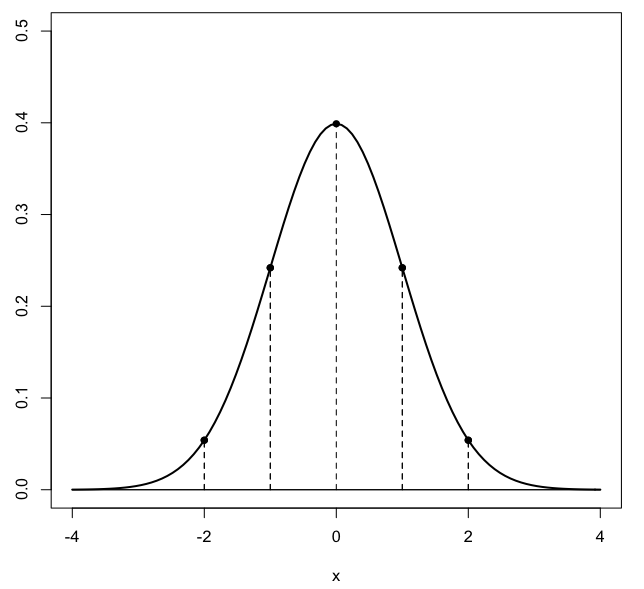
\includegraphics [scale=0.4] {gauss3.png} \end{center}
\begin{document}
\maketitle
\Large
\subsection*{Cauchy' First Integral Theorem}
Cauchy's first theorem says that the integral of an analytic function over a closed path is equal to zero (when the enclosed region is without a singularity).
\[ \oint_C f(z) \ dz = 0 \]
This will turn out to be a consequence of Green's Theorem, which I've written about a lot before.  Let
\[ z = x + i y \]
\[ dz = dx + i dy \]
\[ z = f(x,y) = u(x,y) + iv(x,y) \]
Our integral is
\[ \oint_C z \ dz = \int (u(x,y) + iv(x,y)) \ (dx + i dy) \]
\[ =  \oint_C u(x,y) \ dx - \int v(x,y) \ dy + i \int v(x,y) \ dx + i \int u(x,y) \ dy \]
As before, because we are moving along a curve there is a relationship between $x$ and $y$, so we can either express that relationship or parametrize the curve.  In any case, these become integrals in a single variable.  We remove extra $(x,y)$ notation:
\[ =  \oint_C u \ dx - \int v \ dy + i \int v \ dx + i \int u \ dy \]

\subsection*{proof of Cauchy 1}
Back in vector calculus we proved Green's theorem, which says that for two real functions of $x$ and $y$:  $M(x,y)$ and $N(x,y)$:
\[ \oint_C M dx + N dy = \iint_R (\frac{\partial N}{\partial x} - \frac{\partial M}{\partial y}) \ dx \ dy \]
Back then, $M$ and $N$ were components of a vector field $\mathbf{F}$ and we wrote the shorthand for curl:
\[ = \iint_R \nabla \times \mathbf{F} \ dA\]
but the important thing is that they are real functions of two variables $f: \mathbb{R}^2 \rightarrow \mathbb{R}^1$.

In terms of $u$ and $v$ we have for the real part of Cauchy's Theorem that $M=u$ and $N = -v$ (notice the minus sign!).  

So:
\[ \oint u \ dx - \oint v \ dy = \iint_R (-\frac{\partial v}{\partial x} -  \frac{\partial u}{\partial y}) \ dx \ dy \]
\[ = - \iint_R (v_x + u_y) \ dx \ dy \]
But, according to the CRE
\[ u_y = -v_x \]
Hence, this integral is zero.

For the imaginary part:
\[ \oint v \ dx + \oint u \ dy =  \iint_R (\frac{\partial u}{\partial x} - \frac{\partial v}{\partial y}) \ dx \ dy \]
\[ =  \iint_R (u_x - v_y) \ dx \ dy \]
But, again, according to the CRE
\[ u_x = v_y \]
So the integral for the imaginary part is also zero, and thus the whole thing is zero as well:
\[ \oint u \ dx - \oint v \ dy + i \oint v \ dx + i \oint u \ dy = 0 \]

Remember how important it was (for Green's theorem) that the function being integrated be defined everywhere in the region.  For example, it is \emph{not} true that

\[ \oint_C \frac{1}{z} \ dz = 0 \]

if the curve $C$ includes the origin, but it \emph{is} true otherwise.  A simple demonstration for the former case is the unit circle centered at the origin.  We write
\[ z = r e^{i\theta} \]
\[  \frac{dz}{d\theta} = r i e^{i\theta} = iz \]
Hence
\[ \oint_C \frac{1}{z} \ dz = \oint_C \frac{1}{z} \ iz \ d \theta \]
\[ = i   \oint_C  d \theta = 2 \pi i \]

\subsection*{Cauchy' First Integral Theorem}

Cauchy 1 is a theorem that says the integral of an analytic function over a closed path (over a region without a singularity), is equal to zero.
\[ \oint_C f(z) \ dz = 0 \]
We proved this in the last part.  

We will integrate the function $f(z) = z$ over a rectangle ($R = [0,a] \times [b,0]$.  Write
\[ z = x + i y \]
\[ dz = dx + i dy \]
\[ f(x,y) = u(x,y) + iv(x,y) \]
Our integral is
\[ \int z \ dz = \int (u + iv) \ (dx + i dy) \]
\[ = \int u \ dx - \int v \ dy + i \int v \ dx + i \int u \ dy \]
Since the whole thing is equal to zero over our closed path, both parts are equal to zero:
\[ \int u \ dx - \int v \ dy = 0 \]
\[ \int v \ dx + \int u \ dy \]
Does this look familiar??

\subsection*{application of Cauchy 1}

The function we'll be working with is the one we introduced before:
\[ u(x,y) =  e^{-x^2} e^{y^2} \cos 2xy \]
\[ v(x,y) = e^{-x^2} e^{y^2} (- \sin 2xy) \]
Everything will simplify pretty quickly.  Divide the path into its four parts and compute each separately:
Over $C1$, $y=0$ and $dy = 0$ so we have:
\[ \int_{C1} = \int u \ dx = \int_0^a e^{-x^2} e^{0} \cos 0 \ dx = \int_0^a e^{-x^2} \ dx \]
C2 ($x = a$, $dx = 0)$:
\[ \int_{C2} = - \int_0^b e^{-a^2} e^{y^2} (- \sin 2ay) \ dy  \]
C3 ($y = a$, $dy = 0)$:
\[ \int_{C3} = \int_a^0 e^{-x^2} e^{b^2} (\cos 2bx) \ dx  \]
C4 ($x = 0$, $dx = 0$):
\[ \int_{C4} = \int_b^0 e^{y^2} (-\sin 0) \ dy = 0 \]
So all together:
\[ \int_0^a e^{-x^2} \ dx - \int_0^b e^{-a^2} e^{y^2} (- \sin 2ay) \ dy + \int_a^0 e^{-x^2} e^{b^2} \cos 2bx \ dx = 0 \]
\[ \int_0^a e^{-x^2} \ dx = e^{-a^2} \int_0^b e^{y^2} (- \sin 2ay) \ dy + e^{b^2} \int_0^a e^{-x^2} \cos 2bx \ dx  \]
Let $a \rightarrow \infty$.  Then
\[ e^{-a^2} \rightarrow 0 \]
so the first term on the right side goes to zero and we have:
\[ \int_0^{\infty} e^{-x^2} \ dx = e^{b^2} \int_0^{\infty} e^{-x^2} \cos 2bx \ dx  \]
But we know the value of the left-hand side, it is 
\[ \int_0^{\infty} e^{-x^2} \ dx = \frac{\sqrt{\pi}}{2} \]
so
\[  \int_0^{\infty} e^{-x^2} \cos 2bx \ dx = \frac{\sqrt{\pi}}{2} \ e^{-b^2} \]
The Gaussian that we knew, is a special case of this general form.

\subsection*{derivation of Cauchy 2}
Suppose $f(z)$ is analytic everywhere within some region \emph{except} at a singularity, $z_0$.  For example, suppose we have
\[ \frac{f(z)}{z-z_0} \]
and suppose we integrate this around a special closed path in the region of analyticity:
\[ \oint \frac{f(z)}{z-z_0} \ dz \]
\begin{center} 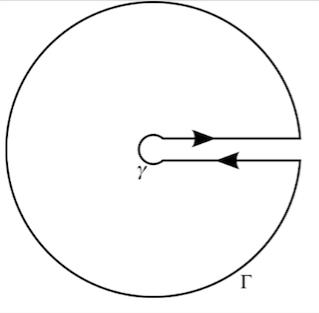
\includegraphics [scale=0.6] {keyhole.png} \end{center}
It's not labeled but the singularity $z_0$ is at the center of the two concentric circles.  The "keyhole" excludes $z_0$ so $f$ is analytic everywhere in the region enclosed by the path, and the total integral is zero by Cauchy's first theorem.  The straight line segments are so close as to be equal, but traversed in opposite directions, so the contribution from them is zero.  Thus we have that the integral around the outer ring counter-clockwise + the integral around the inner ring clockwise add up to zero.

Reversing the direction of integration on the inner ring changes the sign of the value, hence we have that
\[ \oint_{C \ \text{outer}} \frac{f(z)}{z-z_0} \ dz - \oint_{C \ \text{inner}} \frac{f(z)}{z-z_0} \ dz = 0 \]
But we haven't said anything about the radius of these rings.  

What this means is that the value of the integral around a ring enclosing a singularity is not zero, but it has the same value for a ring of \emph{any} radius.  It's independent of the radius.
\[ \oint_{C \ \text{outer}} \frac{f(z)}{z-z_0} \ dz = \oint_{C \ \text{inner}} \frac{f(z)}{z-z_0} \ dz \]

We can parametrize this path by saying that each point on the curve is given by
\[ z = z_0 + \rho e^{i\theta}, \ \ \ 0 \le \theta \le 2 \pi \]
\[ dz = \rho i e^{i \theta} \ d \theta \]
\[ \oint \frac{f(z)}{z - z_0} \ dz = \int_0^{2\pi} \frac{f(z_0 + \rho e^{i\theta})}{\rho e^{i \theta}} \ \rho i e^{i\theta} \ d \theta \]
\[ = i \int_0^{2\pi}  f(z_0 + \rho e^{i\theta}) \ d \theta \]
\[ = i \int_0^{2\pi}  f(z) \ d \theta \]
We may choose $\rho$ as small as we like, and in particular, if we choose it very small ($\rho \rightarrow 0$) we have
\[ f(z) \rightarrow f(z_0) = \text{constant} \]
and since it's constant we can bring it out of the integral!
\[  \oint \frac{f(z)}{z - z_0} \ dz = f(z_0) i \int_0^{2\pi} d \theta \]
\[ = 2 \pi i f(z_0) \]

In previous sections we derived three important theorems about complex functions.  (1) The Cauchy-Riemann equations (CRE) apply to analytic functions---functions that have derivatives---and vice-versa.
\[ u_x = v_y \]
\[ u_y = - v_x \]
We allow analytic functions to have a finite number of isolated singularities or poles where the function may "blow up."

(2) We used the CRE and Green's theorem to show that if a function is analytic everywhere in a simply-connected region, then the integral around any closed path in the region is zero.
\[ \oint f(z) \ dz = 0 \]
(3) On the other hand, if the region contains a singularity or pole, then we used a trick to show that the integral around \emph{any} closed path surrounding the pole has the same value.  This allows us to shrink the curve down to the immediate neighborhood of the pole and leads to the result in the limit as $z \rightarrow z_0$:
\[ \oint_C \frac{f(z)}{z - z_0} \ dz = 2 \pi i f(z_0) \]
(4) We can extend this result to a finite number of poles.  The value of the integral around all of them is the sum of the values for the individual poles.

\end{document}  